%-------------------
%-------------------
\chapter{Einleitung}

Wirbeltiere sind allgegenwärtig. Sie sind nicht nur im alltäglichen Leben anzutreffen, sondern auch in Computerspielen und Filmen. In der Produktion dieser Medien besteht also ein stetiger Bedarf an 3D-Modellen von Wirbeltieren.
Trotzdem gibt es nur wenige Algorithmen, die die KünstlerInnen bei dieser zeitintensiven Arbeit unterstützen \cite{PCGSurvey_videoGames}.\\
Hier wird ein Algorithmus zur Generierung abstrahierter, aber dennoch wirklichkeitsnaher, 3D-Modelle von Skeletten vorgestellt, die die Grundlage für die Modellierung eines kompletten Tieres bilden können.
Viele andere Ansätze generieren hingegen zunächst 3D-Modelle von der "`Außenhaut"' der Tiere und passen dann ein sehr abstraktes Skelett (Rig) für die Animation ein (siehe \mbox{Abschnitt \ref{procedural_generation}}). 
Dieses Rig hat nicht viel mit einem echten Wirbeltierskelett zu tun und ist nur für die Animation gedacht.

% Ziel
Diese Arbeit konzentriert sich auf die Generierung von relativ wirklichkeitsnahen Skeletten, die dann unterschiedlich weiterverwendet werden können.
Einerseits können die Skelette als Inspiration dienen. Sie können einen Anhaltspunkt zu Körperform, Proportionen und zu möglichen Bewegungsabläufen bieten und es kann schnell eine große Auswahl von ihnen generiert werden.
Andererseits können die Skelette eine Grundlage für sehr realistische Modelle sein. Diese Modelle simulieren zusätzlich zum Skelett auch Muskeln und Haut und benötigen deshalb relativ detaillierte Skelettmodelle. \\
In beiden Fällen darf das Modell nicht zu abstrakt sein, da es sonst zu wenig Informationen zum Aufbau des konkreten Tiers liefert.
Ziel ist es also ein Skelett zu generieren, welches genug Knochen enthält um realistisch zu wirken, aber auch nicht zu viele um den Aufwand für die Generierung und die Programmierung des Algorithmus im Rahmen zu halten.

% Warum nur Wirbeliere?
Der hier vorgestellte Algorithmus beschränkt sich auf die Generierung von Wirbeltierskeletten, da deren Aufbau nicht sehr variiert. Natürlich treten trotzdem mehr Unterschiede hervor, je detaillierter die Skelette betrachtet werden.
Deshalb werden abstrahierte Skelette mit vereinfachten und in der Anzahl reduzierter Knochen generiert. Die Grundlagen zur Biologie der Wirbeltiere, die für diese Arbeit notwendig sind, werden in Kapitel \ref{chapter:biology} vorgestellt, die technischen Grundlagen in Kapitel \ref{chapter:basics}.

% Methoden+Aufbau
Im Folgenden werden die wichtigsten Schritte des Algorithmus kurz angerissen, um den Leser durch den Aufbau der Arbeit zu führen. Ein Überblick über den Ablauf des Algorithmus ist in Abschnitt \ref{section:overview} zu finden und Abbildung \ref{intro_pic} gibt einige grafische Einblicke.\\
Die Datengrundlage für den Algorithmus schafft eine \emph{Principal Component Analysis} (Hauptkomponentenanalyse) auf annotierten 2D-Skelett"-bildern (Kapitel \ref{chapter:pca}). Ohne sie wäre es schwer Skelette in einer natürlichen und stabilen Haltung zu generieren.
Die Knochen des Skeletts werden dann mit Hilfe einer kontextfreien Grammatik generiert und gleichzeitig angeordnet (Kapitel \ref{chapter:skeleton_generation}). 
Zum Schluss wird aus existierenden 3D-Modellen von einzelnen Knochen ein 3D-Modell des generierten Skeletts erstellt (Abschnitt \ref{bone_models})).

Prinzipiell generiert der Algorithmus zufällige Skelette. Es können aber auch Benutzereingaben, \zb zur Anzahl der Extremitäten, berücksichtigt oder Variationen zu schon bestehenden Skeletten generiert werden (Kapitel \ref{chapter:additional_features}). \\
Zusätzliche Informationen zu Implementierungsdetails sind in Kapitel \ref{chapter:implementation_detail} zu finden und abgerundet wird die Arbeit mit Fazit und Ausblick in Kapitel \ref{chapter:conclusion}.


 \begin{figure}
  \centering
  \subfloat[Känguru]{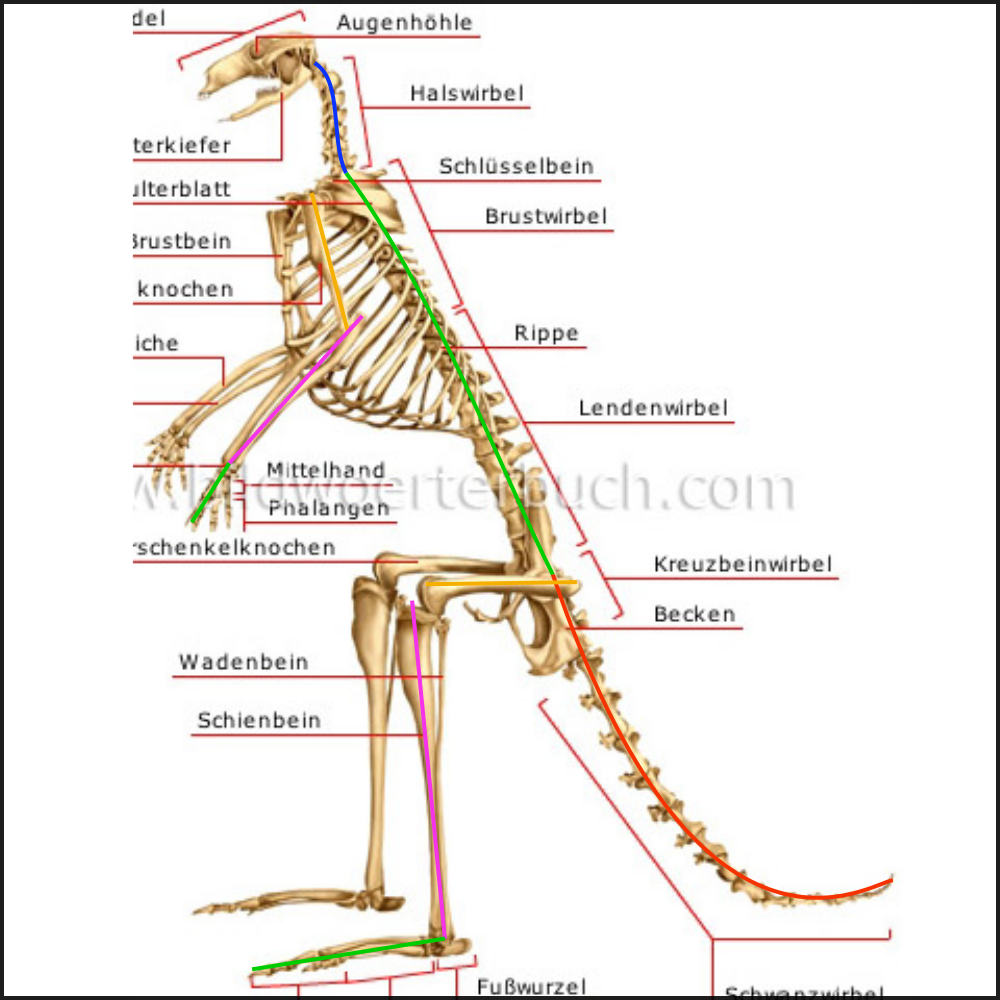
\includegraphics[width=0.32\textwidth]{../PCA/Skelettbilder/Kaenguru_farbig.png}}~
  \subfloat[Klippschliefer]{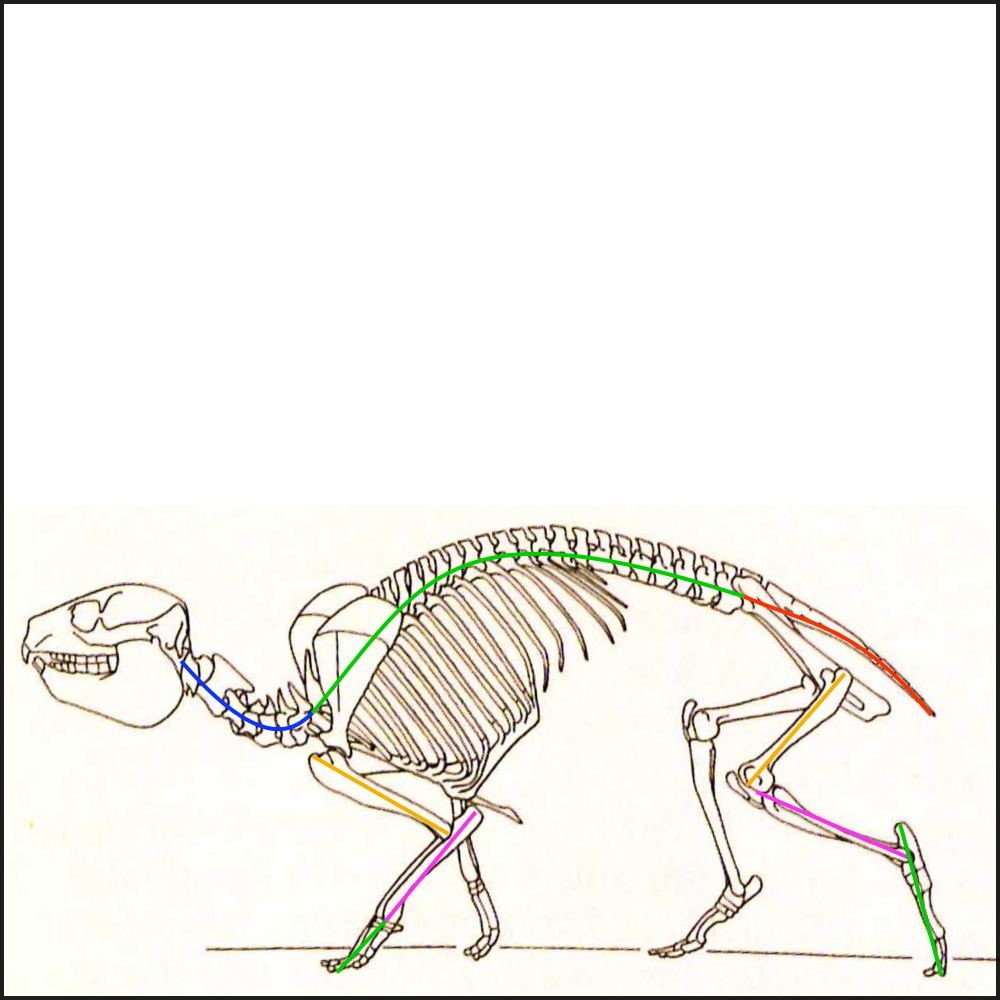
\includegraphics[width=0.32\textwidth]{../PCA/Skelettbilder/Klippschliefer_farbig.png}}~
  \subfloat[Kaninchen]{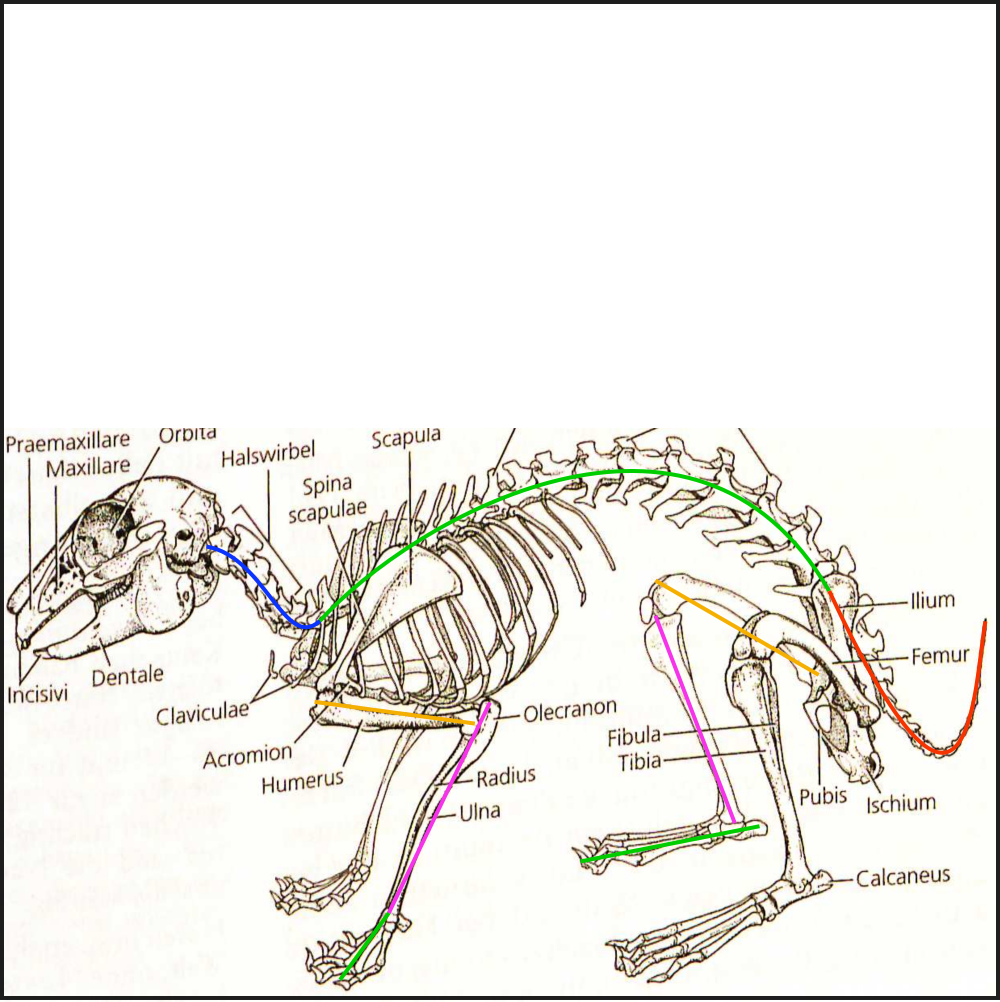
\includegraphics[width=0.32\textwidth]{../PCA/Skelettbilder/Kaninchen_farbig.png}}
  \\
  \subfloat[1. Eigenvektor $-\sigma$]{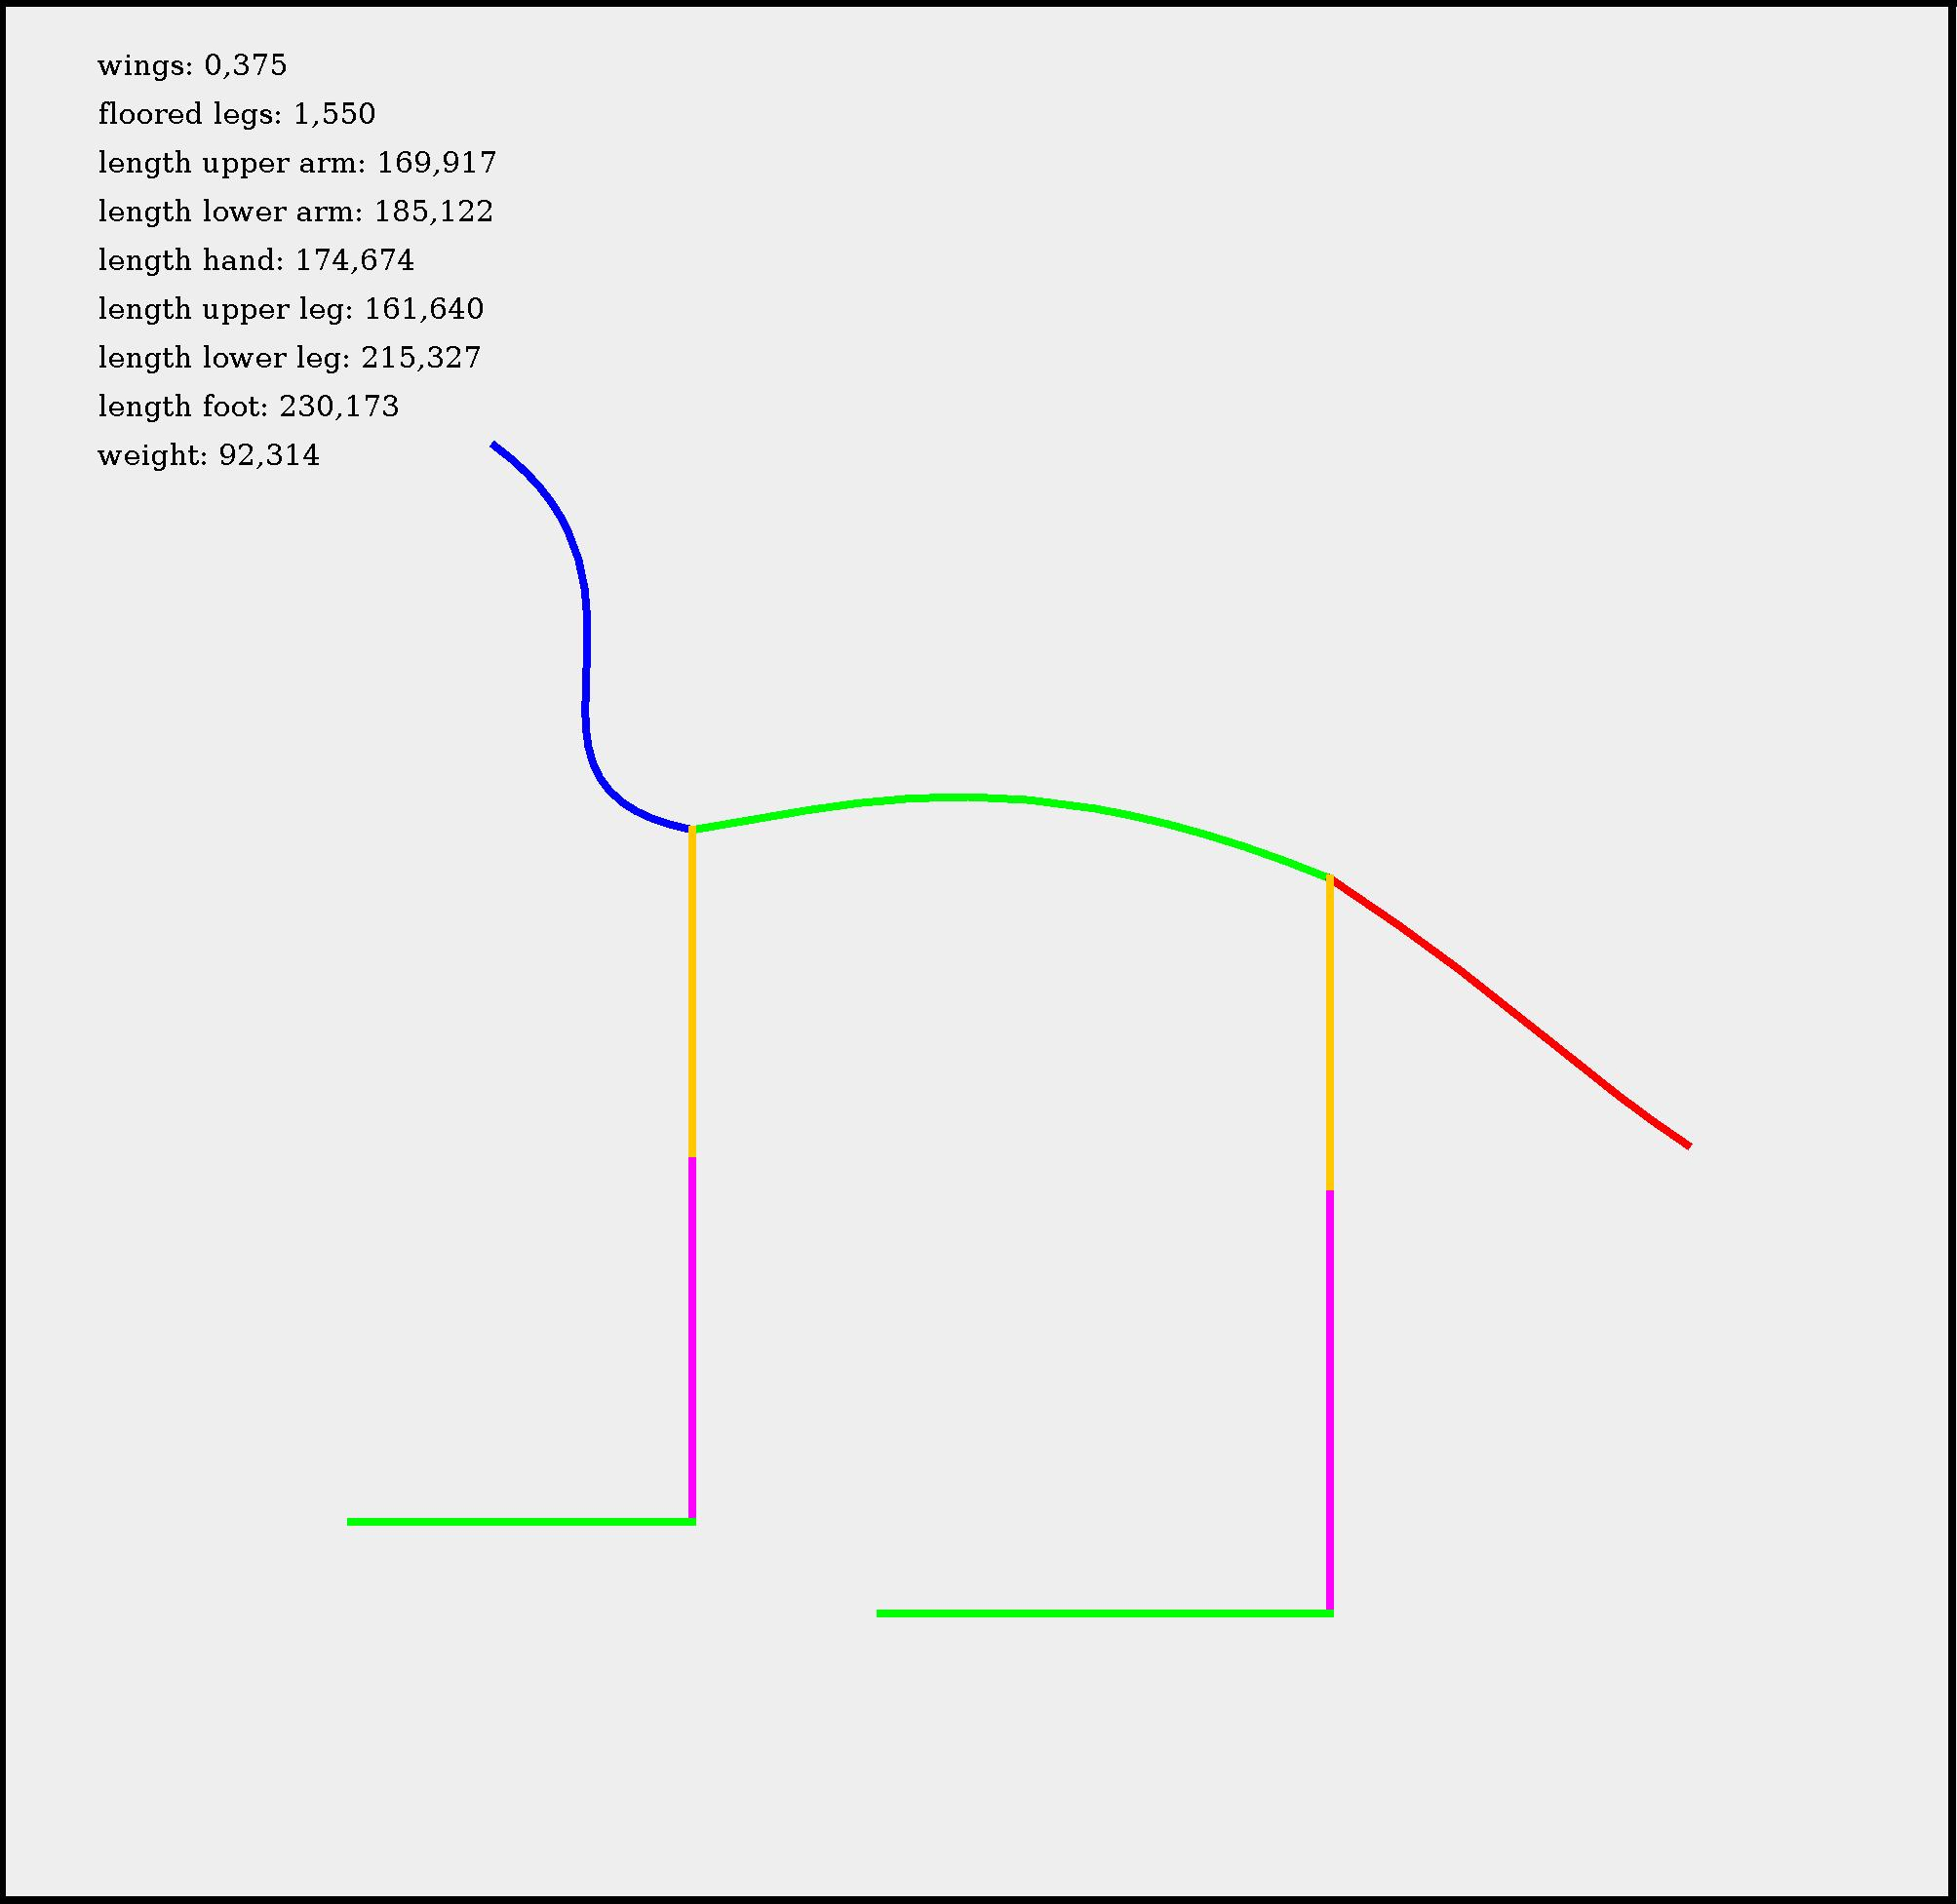
\includegraphics[width=0.32\textwidth]{../PCA/sqrtEV_log_weight_downscaled_wings_legs_and_weight/EV1_neg.jpg}}~
  \subfloat[Mittelwert der Beispiele]{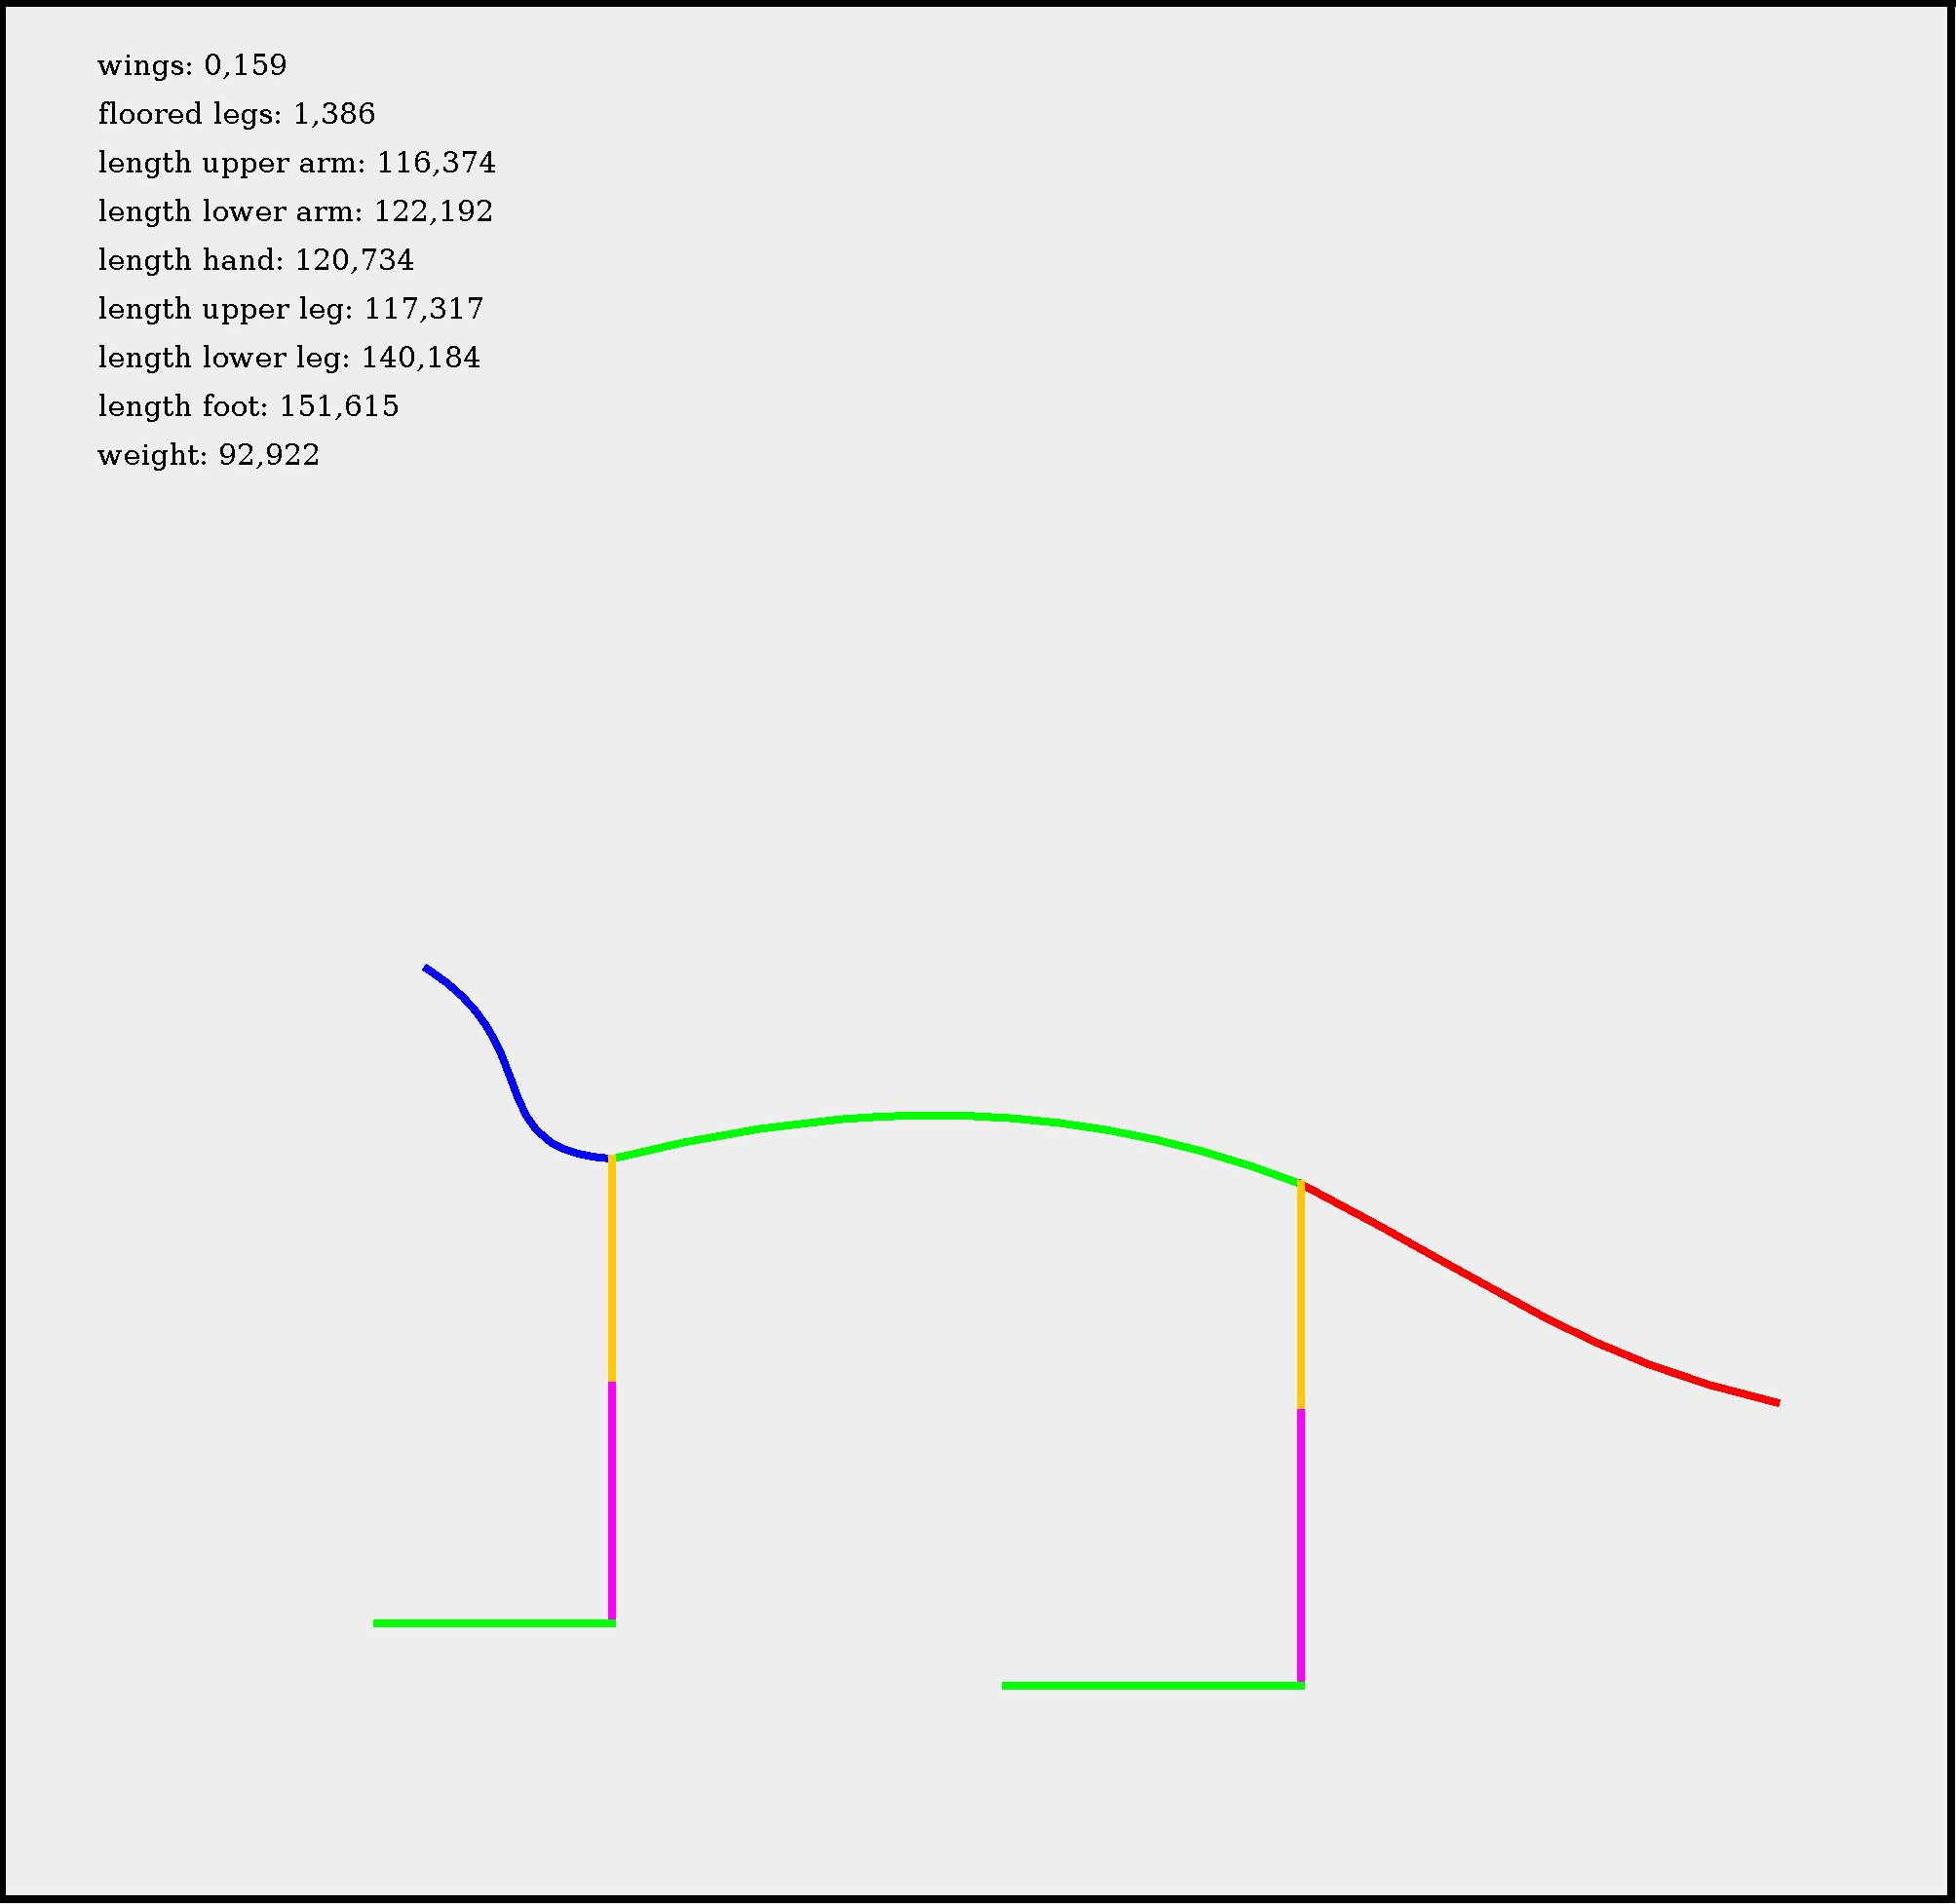
\includegraphics[width=0.32\textwidth]{../PCA/mean_log_weight_downscaled_wings_legs_and_weight(onlyBox,stroke4).jpg}}~
  \subfloat[1. Eigenvektor $+\sigma$]{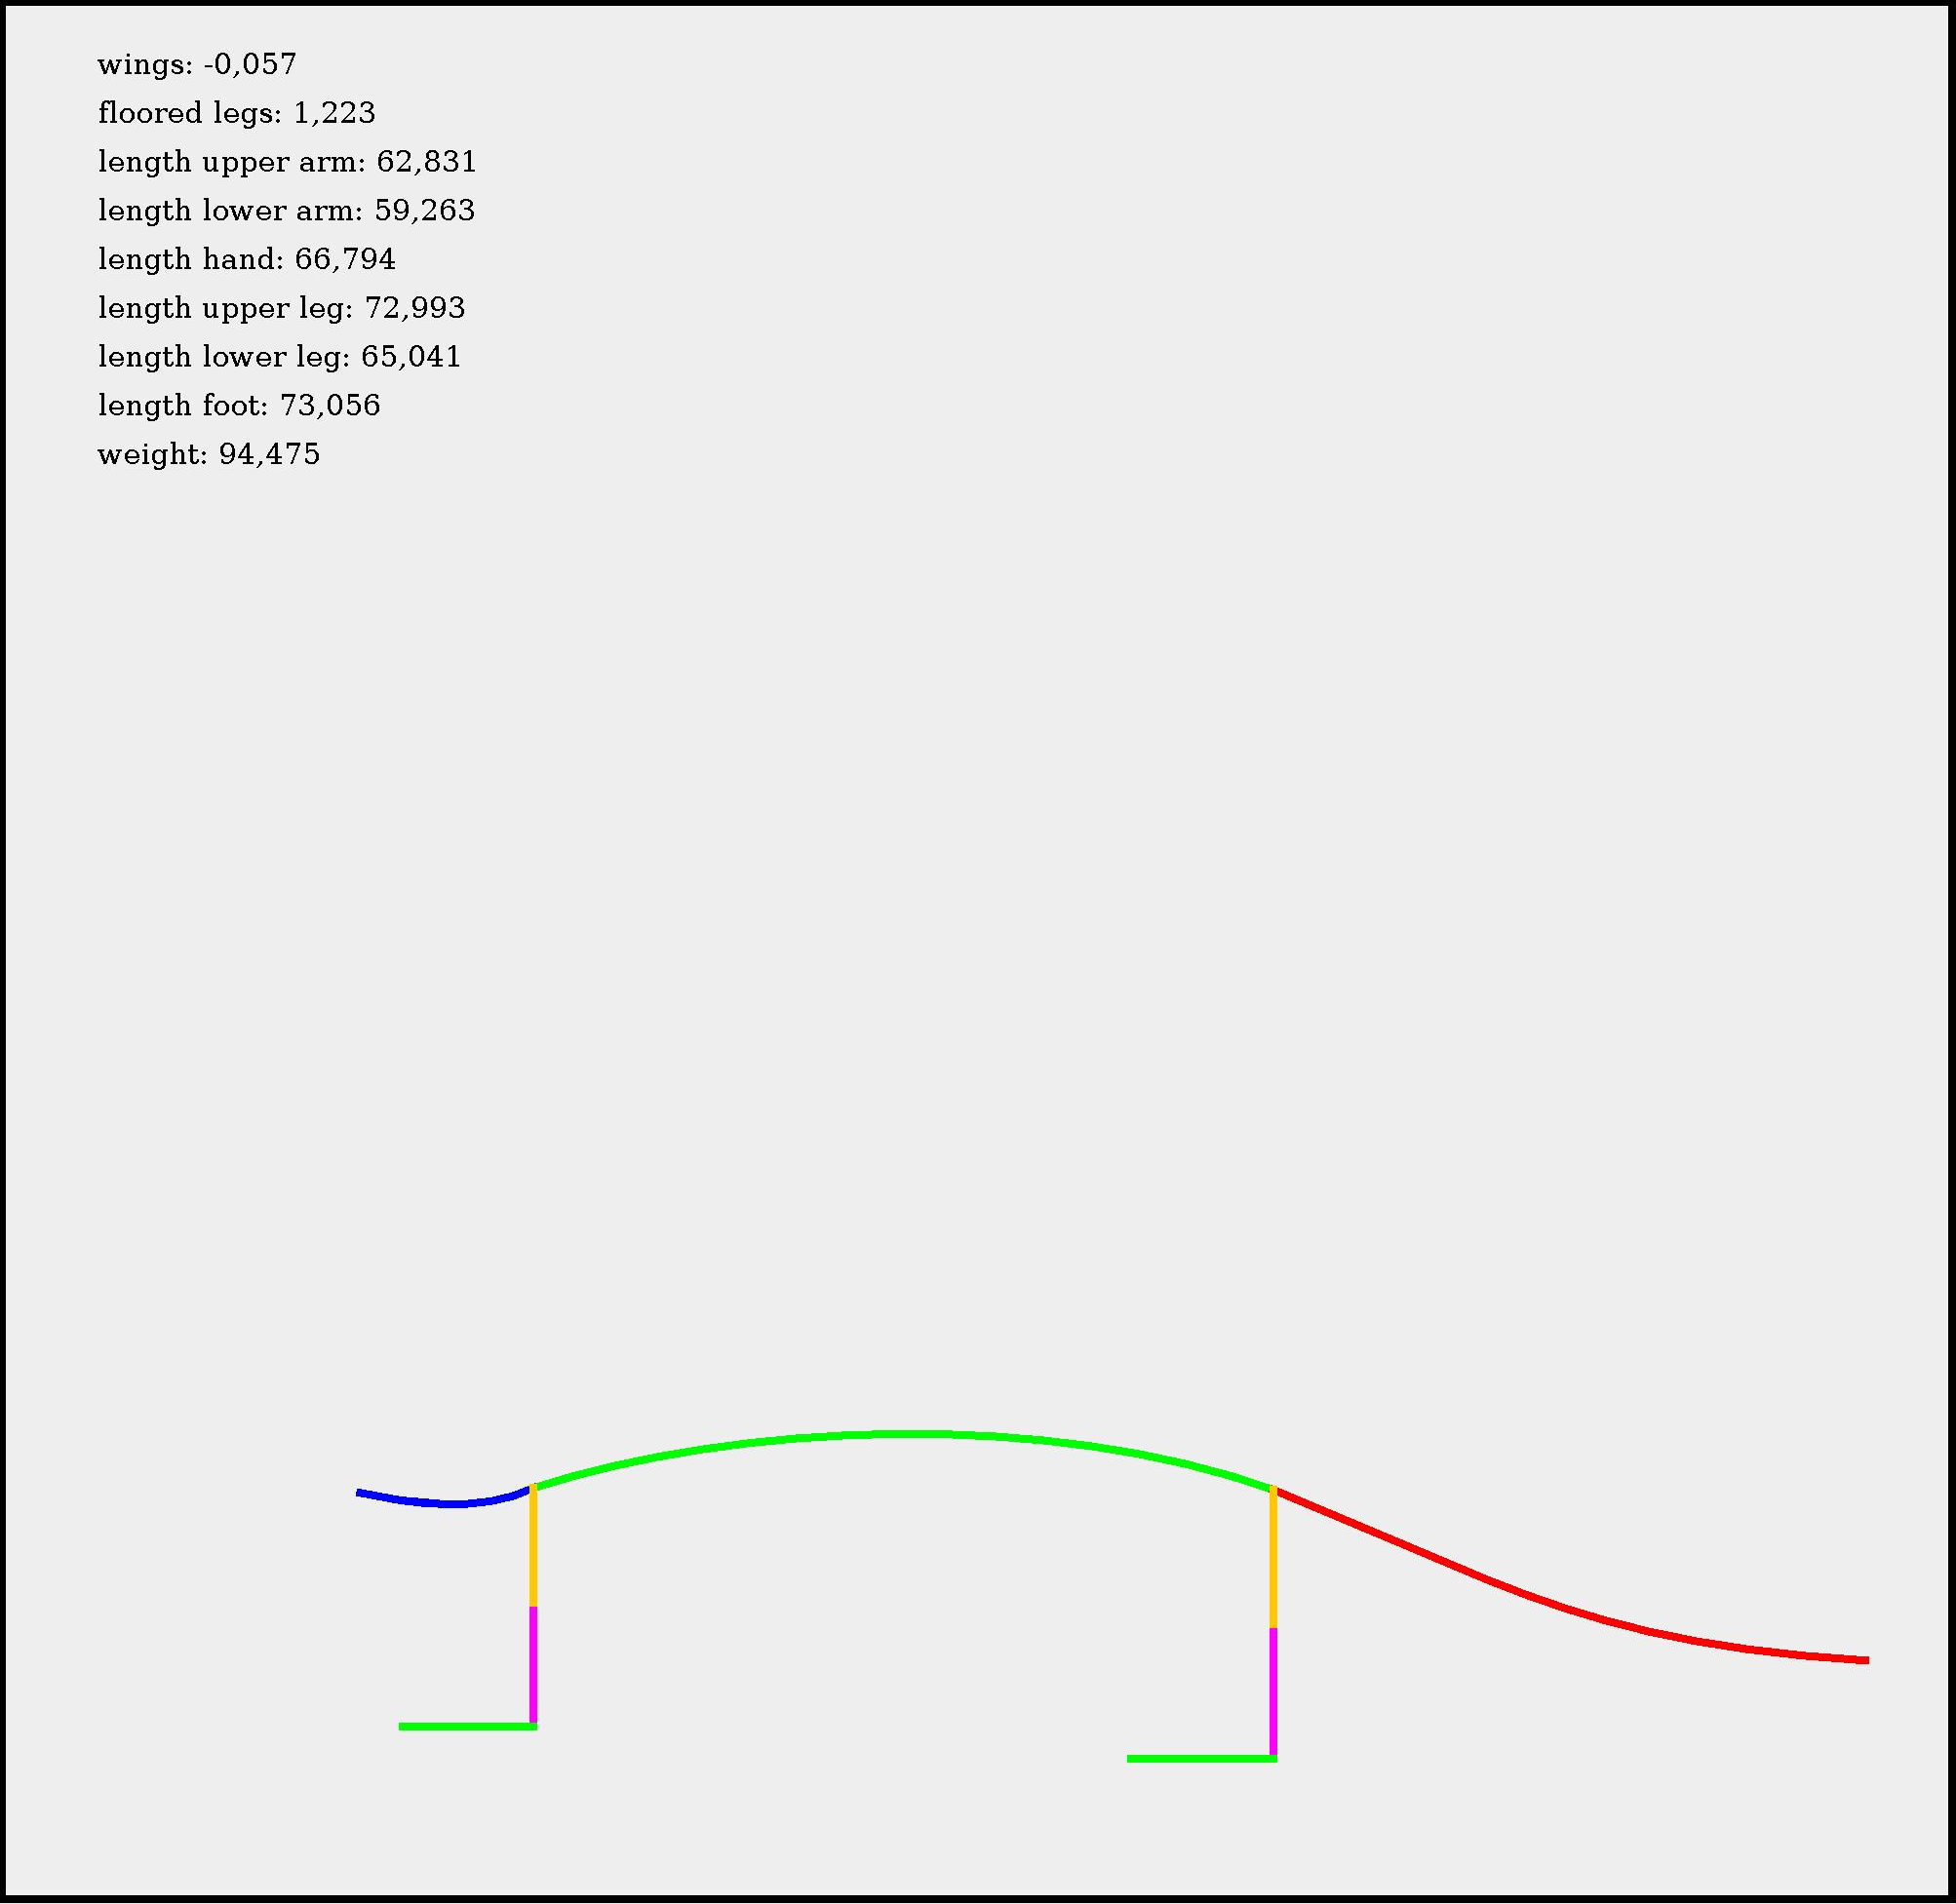
\includegraphics[width=0.32\textwidth]{../PCA/sqrtEV_log_weight_downscaled_wings_legs_and_weight/EV1_pos.jpg}}
  \\
  \subfloat[generiertes Skelett]{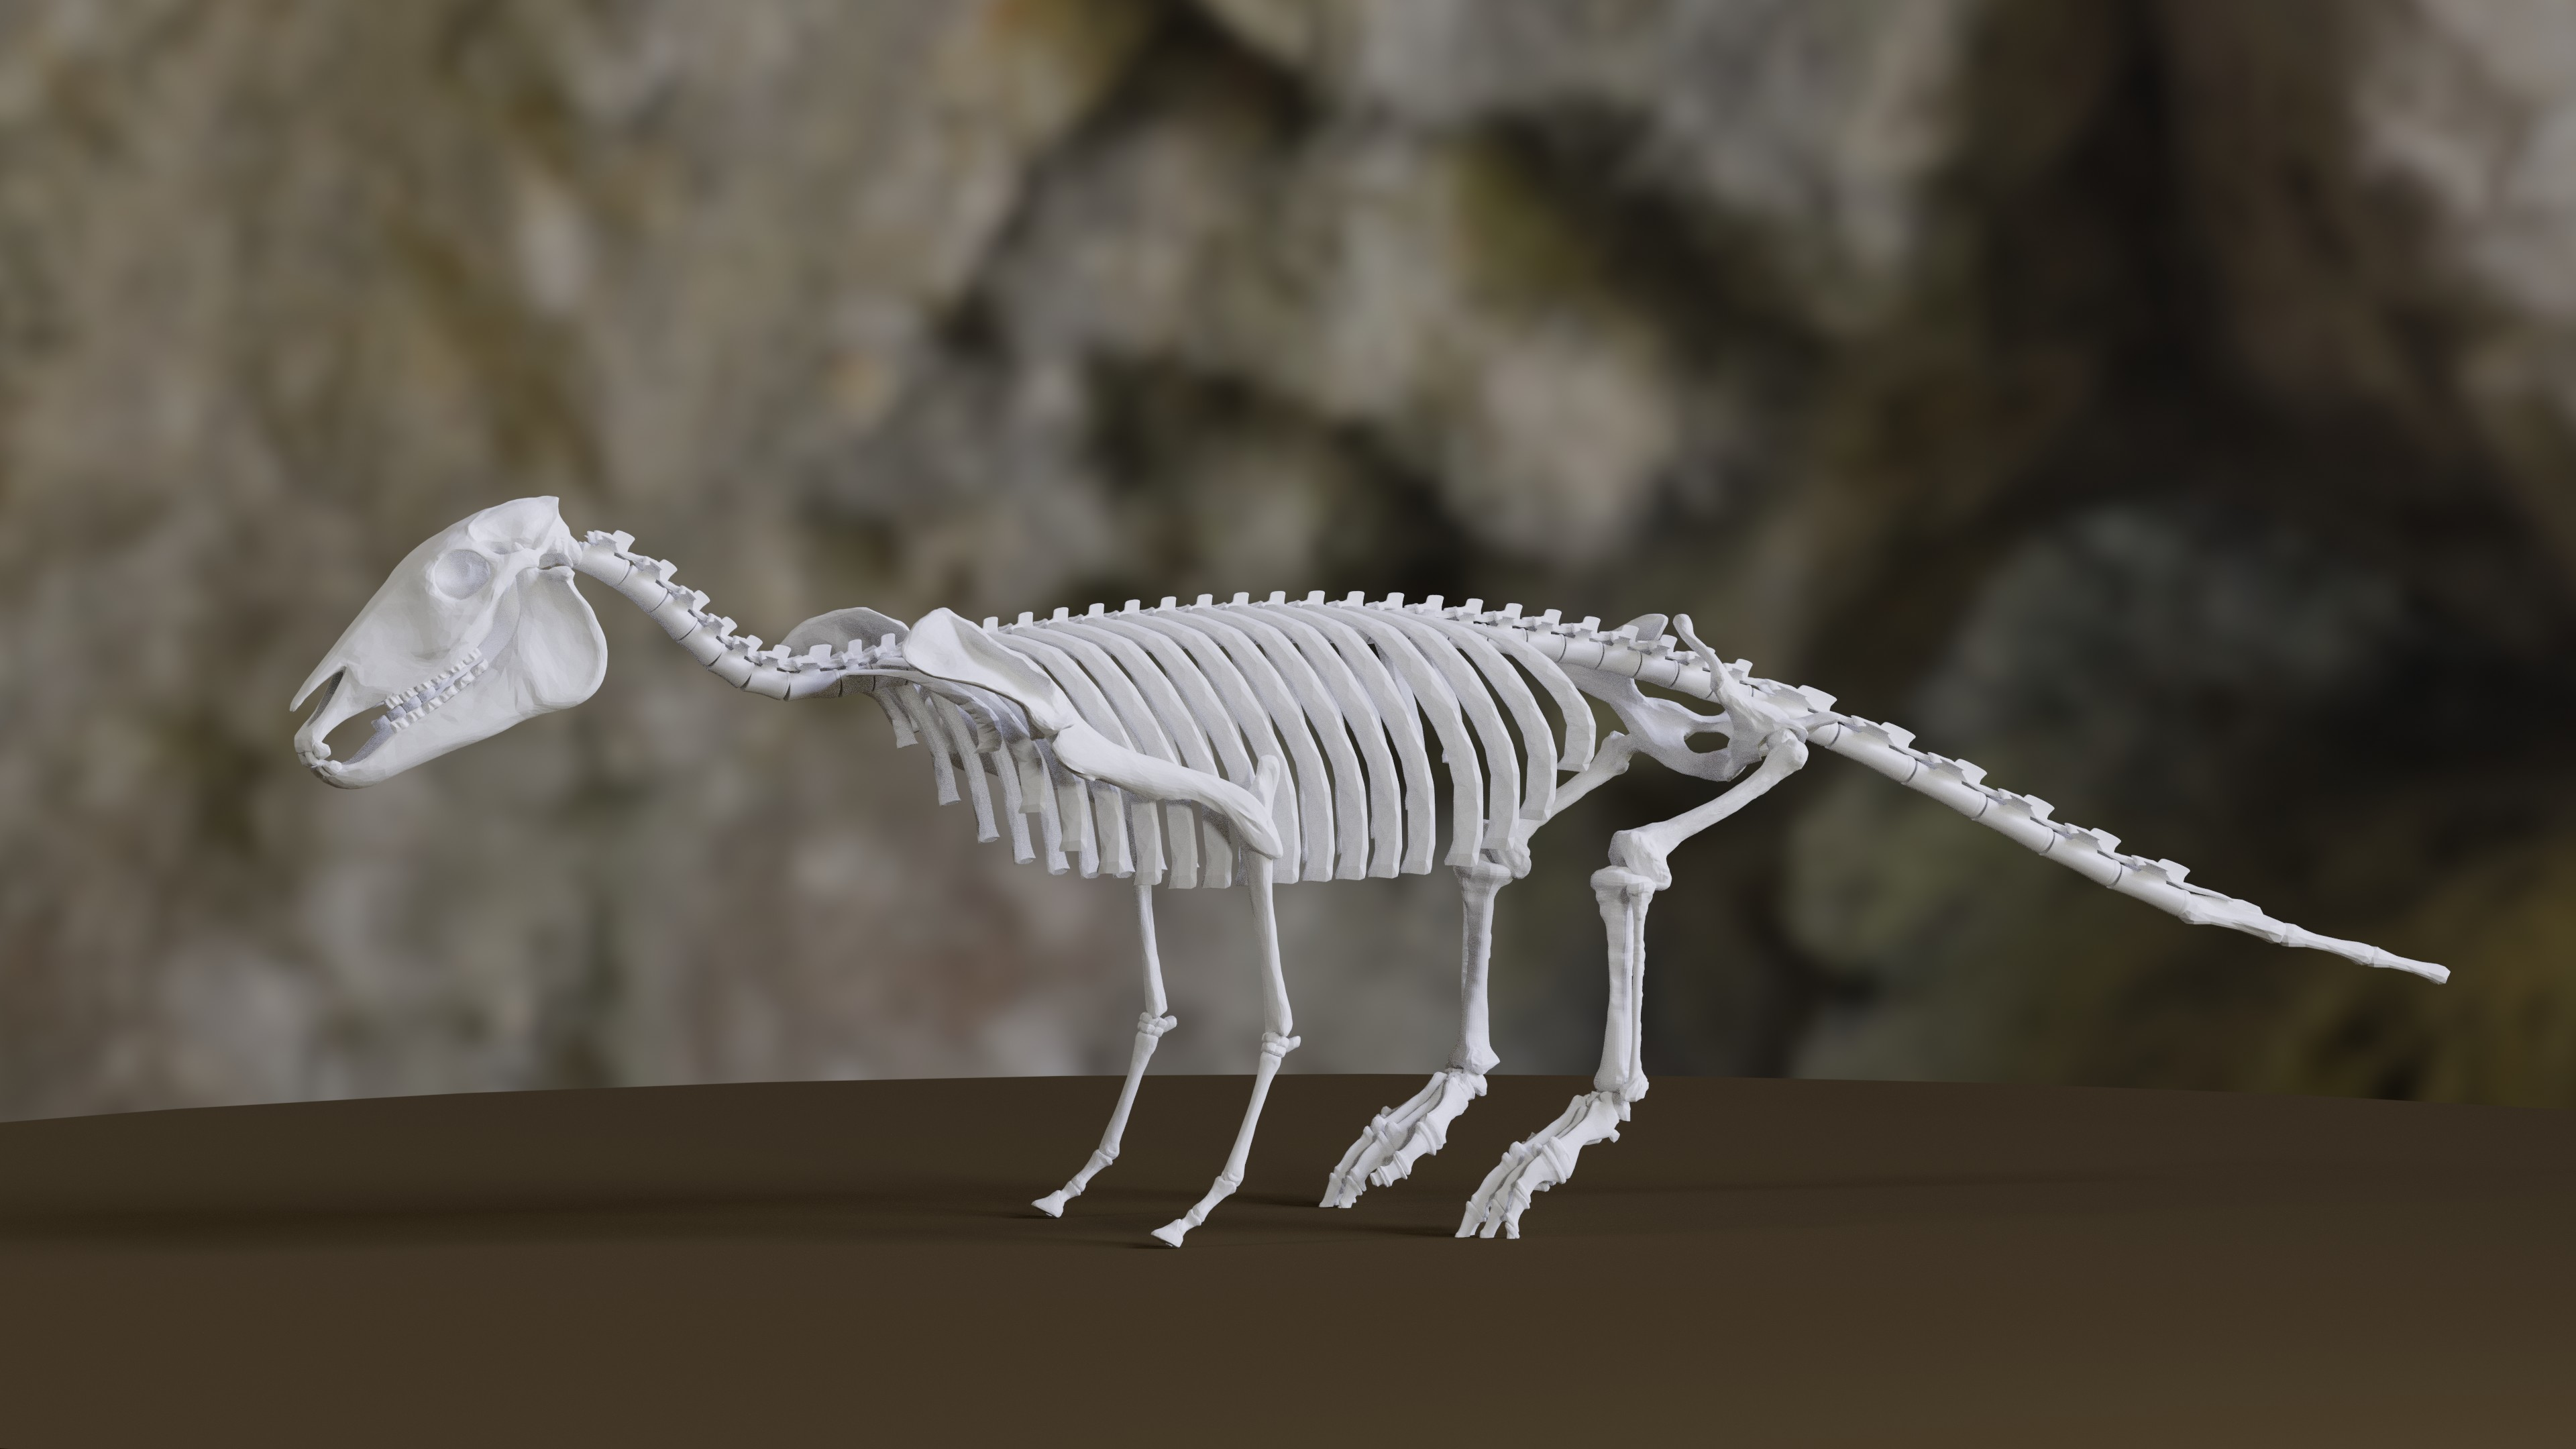
\includegraphics[height=0.25\textheight]{../java_skeleton_generation/example_skeletons/4legs_groundPlane.jpg}}
  
  \caption{(a - c) Beispiele für annotierte Skelette, die als Eingabe für die PCA verwendet wurden. (d - f) Visualisierung der Ergebnise der PCA, (d) ist der Mittelwert der Beispiele, (c) und (e) entstehen jeweils, wenn die Koordinate für den Eigenvektor zum größten Eigenwert die entsprechende positive \bzw negative Standardabweichung annimmt. (g) Beispiel für ein generiertes Skelett (als Hintergrund wurde \cite{background} verwendet).}
  \label{intro_pic}
 \end{figure}
